\documentclass[conference]{IEEEtran}
\usepackage{cite}
\usepackage{graphicx}
\usepackage{booktabs}
\usepackage{hyperref}
\graphicspath{{figures/}}

\begin{document}

\title{Flight Delay Prediction, Phase~2:\\ Can Neural Networks Beat a Simple Baseline?}

\author{}

\maketitle

\begin{abstract}
In Phase~1 we built a simple model, Logistic Regression (LR), that predicts the evening before
whether a New York flight will arrive at least 15 minutes late. In Phase~2 five team members asked
whether neural networks can do better with exactly the same information. We built four models: a
plain neural network, a network that reads the last 14 days of delays in order (a GRU), a network
that learns its own description of each airline and airport, and a mix of a network with XGBoost,
a tree-based model. We also removed one ingredient at a time to see what matters. Every model was
trained and judged under the same rules. None ranked flights better than LR by a margin larger than
chance. Two things did matter: reading the recent days in order, and knowing how busy the timetable
is. The GRU, chosen and locked before the final test, scored 0.399 on the unseen November and
December flights against 0.398 for LR: a tie. The limit is the information available a day ahead,
not the model.
\end{abstract}

\section{Introduction}
Phase~1 found that a day ahead, using only the published timetable and past delays, LR ranks risky
flights about 1.5 times better than random guessing. Neural networks are often better at finding
patterns, so Phase~2 asks one question: \emph{with the same day-ahead information, does a neural
network predict delays better than LR?}

Each team member built one part:
\begin{itemize}
  \item \textbf{Member~1:} a plain neural network, the starting point.
  \item \textbf{Member~2:} a GRU, a network that reads the last 14 days of delays in order.
  \item \textbf{Member~3:} a network that learns a short description of each airline, airport and
  route (``embeddings'').
  \item \textbf{Member~4:} tests that remove one ingredient at a time, and a network--XGBoost mix.
  \item \textbf{Member~5:} one shared evaluation of all models, and the final test.
\end{itemize}

\textbf{How we measure.} Our main measure is the \emph{ranking score} (average precision, often
called PR-AUC). It asks: if we sort flights from most to least risky, how
well do the truly delayed flights rise to the top? Higher is better, and random guessing scores
the share of delayed flights. We also measure the \emph{calibration gap} (expected calibration
error): when a model says ``30\% chance of delay'', how far is that from
what really happens? Lower is better.

\section{The Rules: A Fair Test}
\label{sec:rules}
We use the same 2013 New York flights dataset as Phase~1. Every model used
the same 59 pieces of information as Phase~1: the flight's schedule, airline,
airports, how busy the timetable is, and how delayed recent flights were. Nothing that happens on
the day of travel is used. The year was split by month, and each part had one job
(Fig.~\ref{fig:timeline}):

\begin{itemize}
  \item \textbf{January--July} (188{,}971 flights): the models learn.
  \item \textbf{August} (28{,}756 flights): we pick each model's settings.
  \item \textbf{January--August} (217{,}727 flights): the chosen model learns once more.
  \item \textbf{September--October} (55{,}628 flights, 15.7\% delayed): all models are compared
  on exactly the same flights.
  \item \textbf{November--December} (53{,}991 flights): the final test, opened once, for one model
  only.
\end{itemize}

\begin{figure}[htbp]
\centering
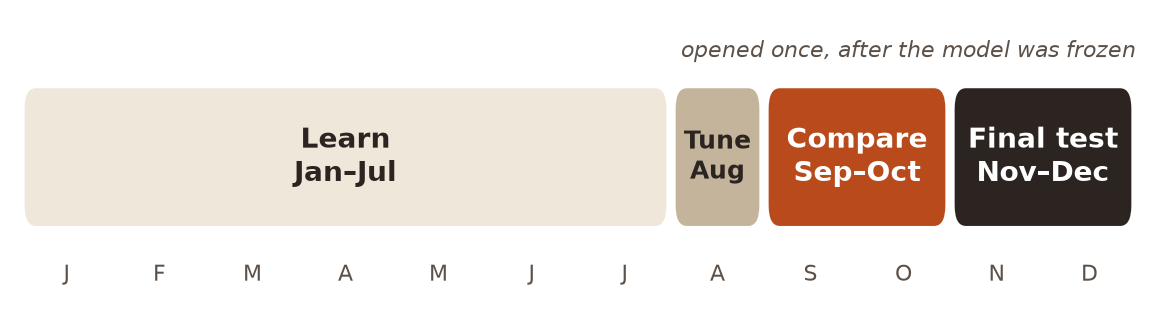
\includegraphics[width=\columnwidth]{fig1_timeline.png}
\caption{Each part of the year has one job. The test months were opened only once, after the final
model was locked.}
\label{fig:timeline}
\end{figure}

\textbf{Is a difference real?} Neural networks give slightly different results each time they are
trained, so every model was trained five times and we report the average. Two models can also
differ by luck. To check, we re-drew the 61 comparison days at random 1{,}000 times and recomputed
the difference each time. This gives a range the difference could
plausibly take. If the range does not include zero, we call the difference \emph{real}. Each
member wrote their plan down before training, so results could not change the plan.

\section{The Four Models}

\textbf{Plain network (Member~1).} A standard neural network~\cite{lecun2015deep} with two hidden layers. Each airline,
airport and route is turned into its own on/off column, giving 1{,}015 inputs. It was trained with
the Adam method and dropout, which switches
off random parts of the network to stop it memorising.

\textbf{GRU over daily delays (Member~2).} For a flight on a given day, this model looks at the
previous 14 days, from oldest to newest (Fig.~\ref{fig:gru}). For each day it sees how delayed the
whole system, the departure airport, the airline and the destination were, and how many flights
there were. A GRU~\cite{cho2014gru} is a network built to read sequences in order. Its summary is
combined with the flight's own details. A past flight only counts once its result was known
(landing plus 30 minutes), so the model never sees information it would not have had. Six
settings were tried (7, 14 or 28 days; two sizes); all scored between 0.368 and 0.372 on August,
and 14 days won.

\begin{figure}[htbp]
\centering
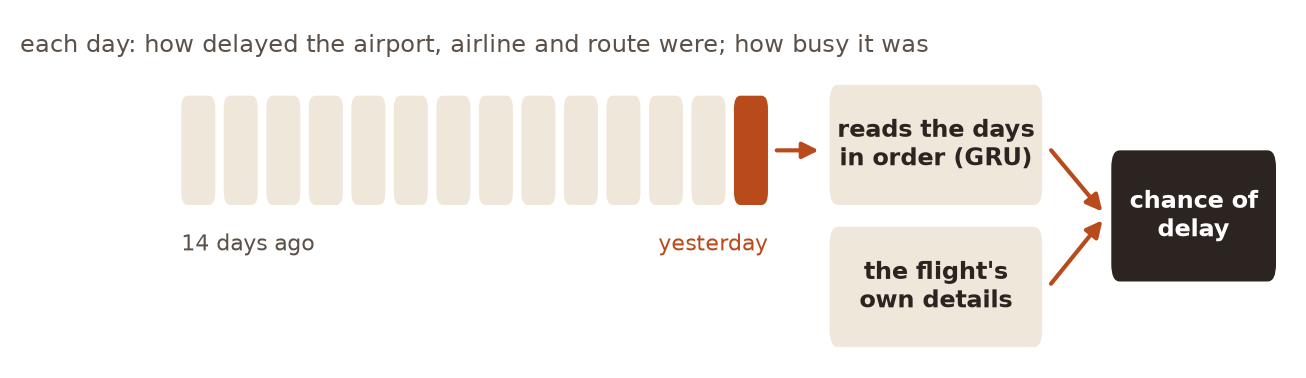
\includegraphics[width=\columnwidth]{fig5_gru_idea.png}
\caption{The GRU reads the last 14 days in order, then combines what it learned with the flight's
own details to give a chance of delay.}
\label{fig:gru}
\end{figure}

\textbf{Embedding network (Member~3).} Instead of hundreds of on/off columns, this network learns
a few numbers that describe each airline, airport and route~\cite{guo2016entity}. The input
shrinks from 1{,}015 to 86 numbers, about 12 times smaller. Member~3 tried 48 combinations of
settings; all scored between 0.391 and 0.397 on August, so the settings barely mattered.

\textbf{Network--XGBoost mix (Member~4).} XGBoost~\cite{chen2016xgboost} builds many small decision
trees. The mix takes 64 numbers learned inside Member~3's network, adds the 49 numeric inputs, and
gives them to XGBoost. The hope was that trees would find patterns the network missed. For a fair
comparison, Member~4 also retrained a plain XGBoost under the same rules.

\section{Results}

\subsection{Overall: nobody beats the baseline}
Fig.~\ref{fig:overall} and Table~\ref{tab:main} show all models on the same September--October
flights. The GRU has the highest average score, 0.295, against 0.290 for LR. But the difference,
+0.005, could plausibly be anywhere from $-0.014$ to $+0.024$, so it is not real
(Fig.~\ref{fig:diff}). The plain network ties LR. The embedding network, plain XGBoost and the mix
are really lower.

\begin{figure}[htbp]
\centering
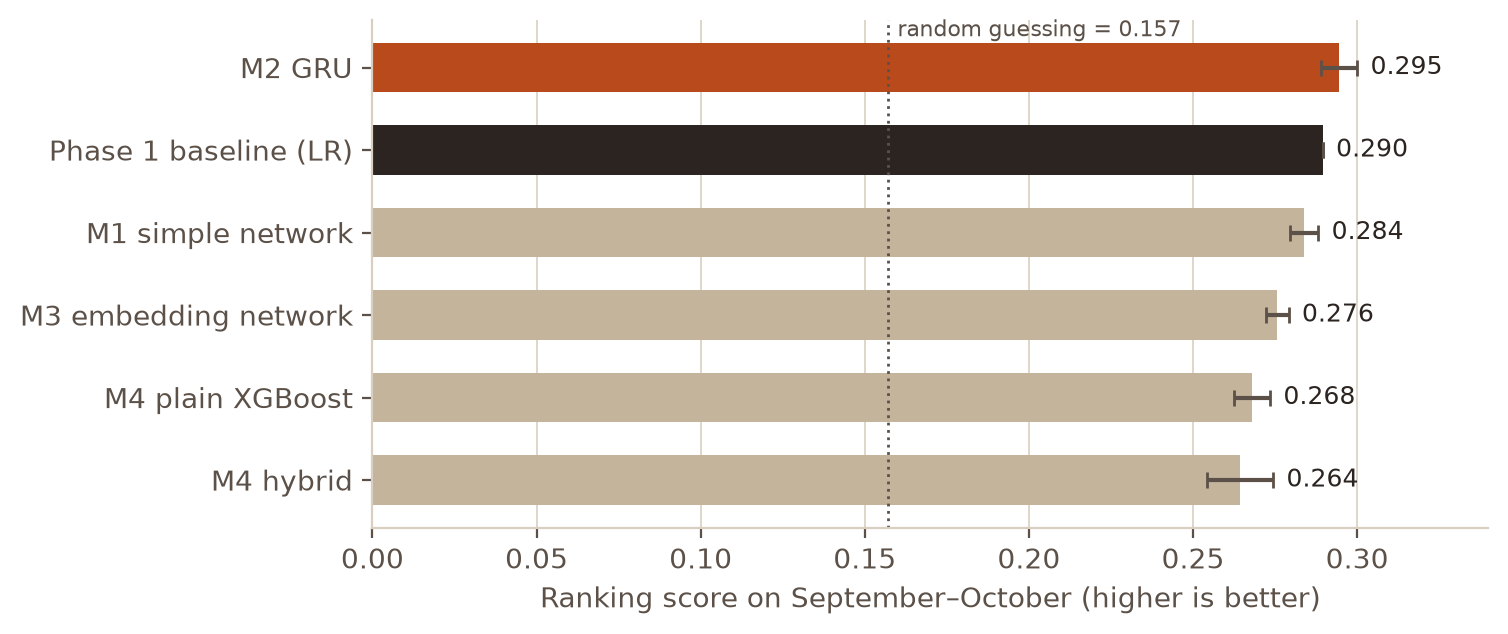
\includegraphics[width=\columnwidth]{fig2_overall.png}
\caption{Ranking score on September--October, average of five runs (lines show the spread). All
models are close; random guessing scores 0.157.}
\label{fig:overall}
\end{figure}

\begin{table}[htbp]
\centering
\caption{September--October results (55{,}628 flights). Difference from LR with its plausible
range; * marks a real difference.}
\label{tab:main}
\resizebox{\columnwidth}{!}{%
\begin{tabular}{lcc}
\toprule
Model & Ranking score & Difference from LR \\
\midrule
LR (Phase~1 baseline) & 0.290 & --- \\
M2 GRU & \textbf{0.295} & +0.005 [$-$0.014, +0.024] \\
M1 plain network & 0.284 & $-$0.006 [$-$0.024, +0.012] \\
M3 embedding network & 0.276 & $-$0.014 [$-$0.022, $-$0.003]* \\
M4 plain XGBoost & 0.268 & $-$0.022 [$-$0.038, $-$0.004]* \\
M4 network--XGBoost mix & 0.264 & $-$0.025 [$-$0.039, $-$0.010]* \\
\bottomrule
\end{tabular}}
\end{table}

\begin{figure}[htbp]
\centering
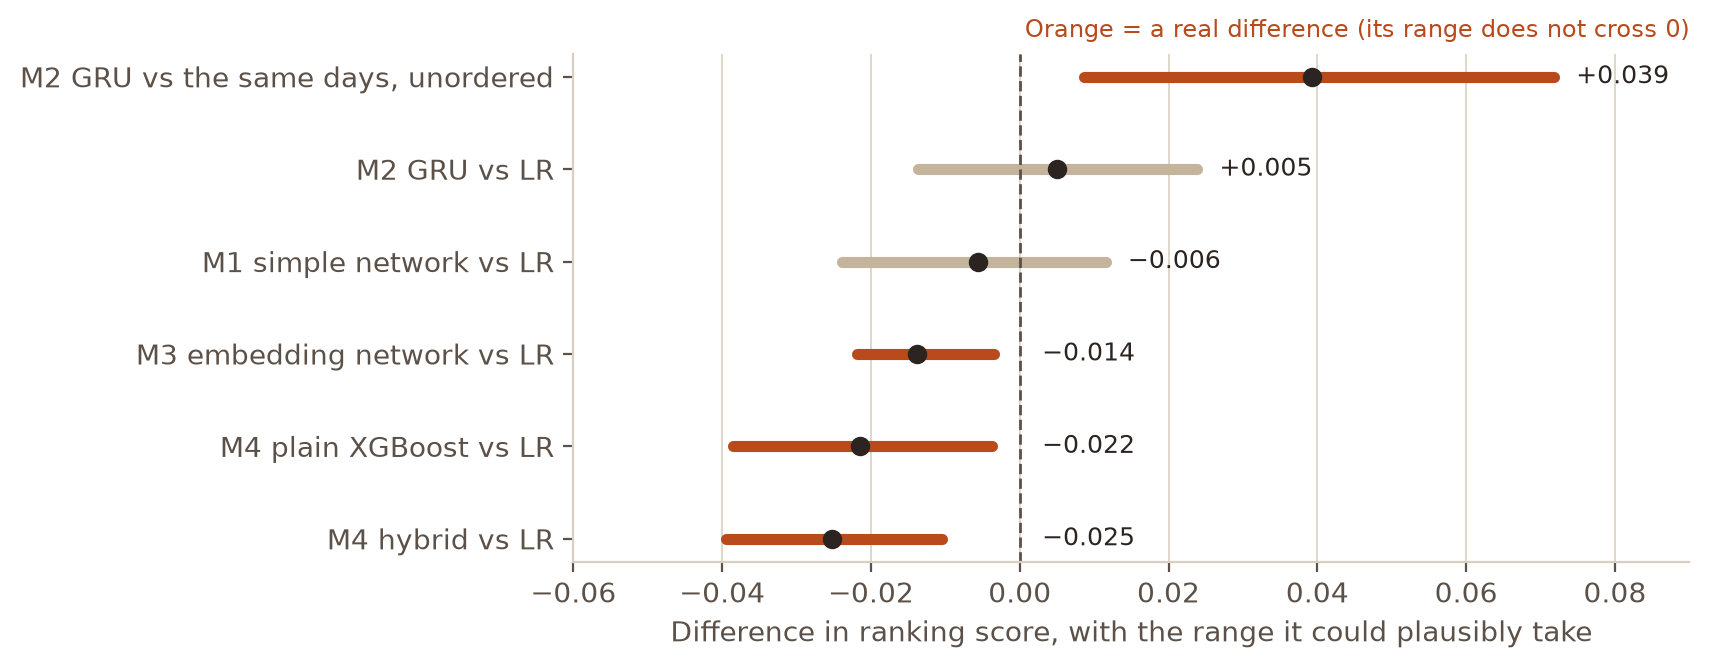
\includegraphics[width=\columnwidth]{fig3_differences.png}
\caption{Each dot is a difference; each bar is the range it could plausibly take. Only orange bars
stay clear of zero.}
\label{fig:diff}
\end{figure}

\subsection{Member~1: the plain network learns fast, then memorises}
On August, the plain network did best after a single pass through the training data (0.380) and
got worse after that, falling to 0.339 by the fourth pass (Fig.~\ref{fig:mlp}). It had started to
memorise the training months instead of learning general patterns, so all five runs stopped after
one pass. On September--October it scored 0.284 against 0.290 for LR, a tie (difference $-0.006$,
range $-0.024$ to $+0.012$). Its probabilities were more honest than LR's before any correction
(calibration gap 0.073 against 0.227).

\begin{figure}[htbp]
\centering
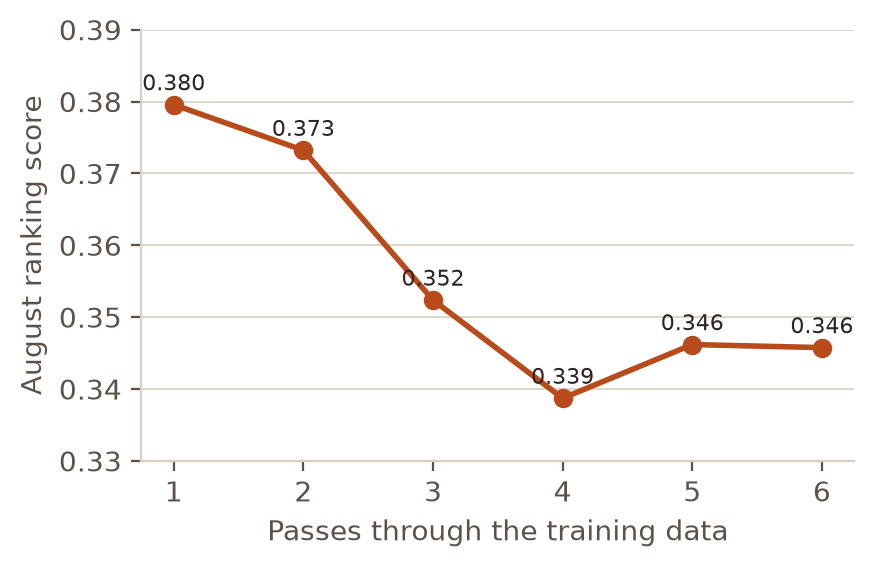
\includegraphics[width=0.8\columnwidth]{fig4_mlp_learning.png}
\caption{Member~1's network on August: best after one pass, then worse as it memorises.}
\label{fig:mlp}
\end{figure}

\subsection{Member~2: the order of recent days matters}
The GRU scored 0.295. To test whether \emph{reading the days in order} helps, Member~2 built a
copy that receives the same 14 days of numbers all at once, without any order. That copy scored
only 0.255, and the GRU beat it by +0.039 (range +0.009 to +0.072): a real difference. So the
order of recent delays carries useful information. The GRU was also ahead of the plain network
by +0.011 (range $-0.000$ to +0.022), just at the edge of being real. Finally, when the 29
hand-made past-delay inputs were removed, the GRU changed by only $-0.006$ (range $-0.022$ to
+0.008): it learns that information from the 14 days by itself.

\subsection{Member~3: settings barely matter}
The embedding network scored 0.276, and every one of its five runs was below LR. Its difference
from LR, $-0.014$ (range $-0.022$ to $-0.003$), is real. Its strength was honest probabilities:
before any correction, its calibration gap was the smallest of all models (0.039).

\subsection{Member~4: what really matters}
Member~4 retrained Member~3's network four times, each time with one ingredient removed
(Fig.~\ref{fig:ablation}). Only removing the four \emph{timetable busyness} inputs (how many
flights the timetable puts at that airport and hour) caused a real drop: $-0.016$ (range $-0.027$
to $-0.006$). Removing the 29 past-delay inputs lowered the score by about as much on average
($-0.018$), but the range ($-0.046$ to +0.006) was too wide to call it real. Using on/off columns
instead of learned descriptions, or removing dropout, changed nothing.

\begin{figure}[htbp]
\centering
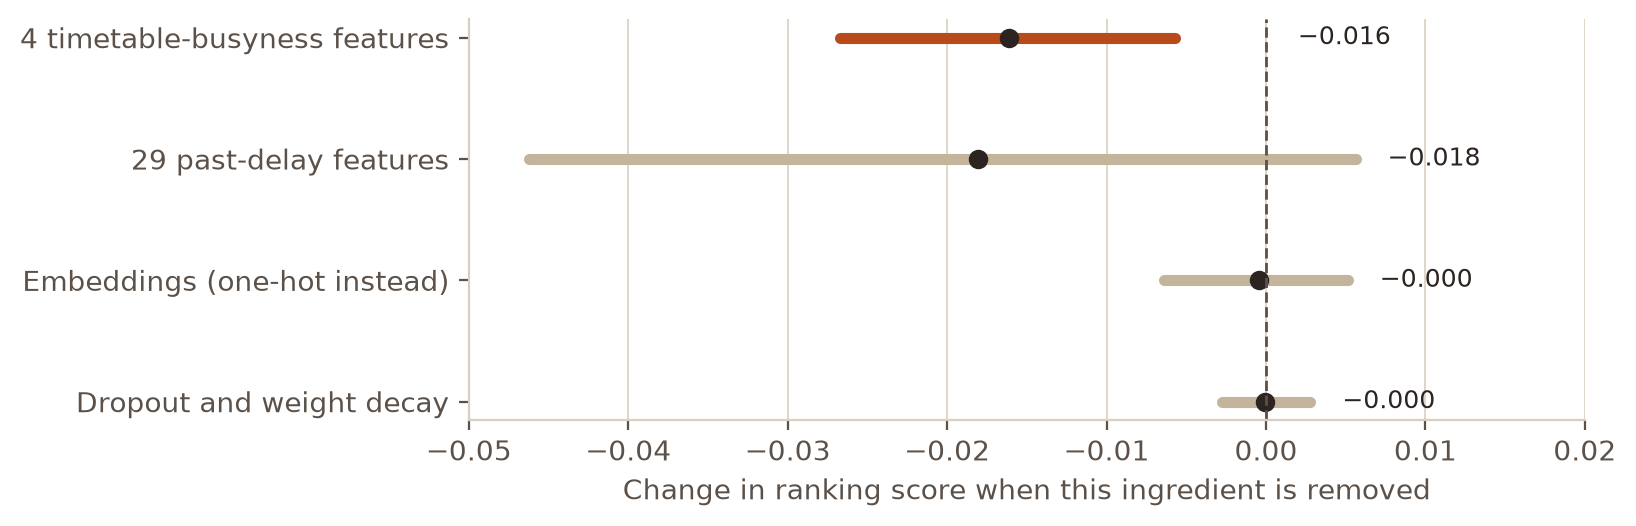
\includegraphics[width=\columnwidth]{fig6_ablation.png}
\caption{Change in score when one ingredient is removed. Only timetable busyness causes a real
drop.}
\label{fig:ablation}
\end{figure}

The network--XGBoost mix scored 0.264, no better than plain XGBoost (difference $-0.004$, range
$-0.017$ to +0.008), and both were really below LR. XGBoost stopped adding trees early (between 3
and 202 trees), a sign that the learned numbers held little extra information.

\subsection{Member~5: honest probabilities and where models struggle}
Most models' raw chances of delay were off. Member~5 corrected each one with a simple adjustment
learned on September~\cite{niculescu2005predicting} and checked it on October
(Fig.~\ref{fig:calib}). After correction, every model's calibration gap fell to between 0.014 and
0.033. The GRU was the most honest (0.014, against 0.027 for LR).

\begin{figure}[htbp]
\centering
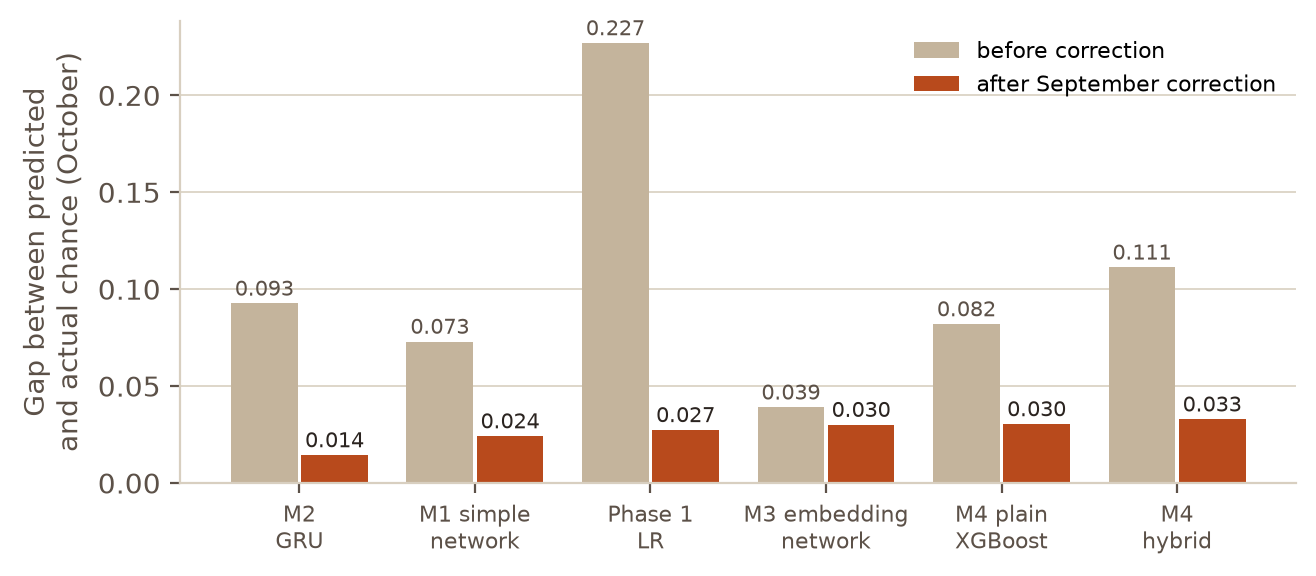
\includegraphics[width=\columnwidth]{fig7_calibration.png}
\caption{Calibration gap on October, before and after the September correction (lower is better).}
\label{fig:calib}
\end{figure}

\textbf{A 60\% alarm.} Planners only want a warning when at least 60\% of warned flights are really
delayed. Using October to set the alarm level, LR and the embedding network could never reach 60\%.
The GRU reached it in all five runs, warning about 160 to 358 October flights. The plain network
also reached it in all five runs, but some runs warned about a single flight. XGBoost and the mix
reached it in only some runs, warning at most 35 and 39 flights, which is not useful.

\textbf{Where models struggle.} Busy groups naturally get higher ranking scores, so Member~5
compared groups by how many times better than random each one is. The hardest airline was FL
(1.28 times random, but only 234 October flights), then AA (1.41). The hardest airport was JFK
(1.53, against 1.86 for EWR). The hardest departure times were 6~a.m.\ (1.35) and 7~p.m.\ (1.36).
After correction, every model still under-predicted delays for flights leaving between 3~p.m.\ and
9~p.m.

\section{The Final Test}
The GRU was chosen for the final test because it had the highest score, the most honest
probabilities and the only useful 60\% alarm on September--October. Before anyone looked at
November and December, the choice was written down and locked: the trained model, its September
correction and its October alarm level. Member~5 then checked that the model reproduced its
earlier September--October predictions exactly, and scored the test months once.

\begin{figure}[htbp]
\centering
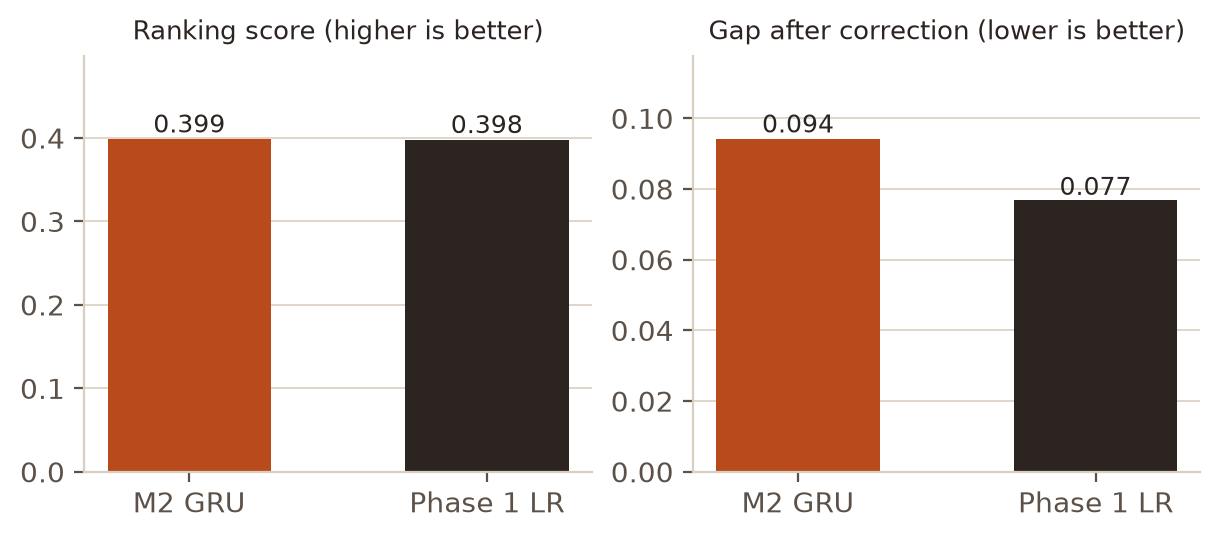
\includegraphics[width=\columnwidth]{fig8_final_test.png}
\caption{Final test on November--December (53{,}991 flights, 25.8\% delayed): the GRU and LR rank
flights equally well.}
\label{fig:test}
\end{figure}

\begin{table}[htbp]
\centering
\caption{Final test, November--December, scored once}
\label{tab:test}
\begin{tabular}{lcc}
\toprule
 & M2 GRU & LR (Phase~1) \\
\midrule
Ranking score & 0.399 & 0.398 \\
Calibration gap, after correction & 0.094 & 0.077 \\
Flights warned at the 60\% alarm & 1{,}102 (2.0\%) & none set \\
Share of warnings truly delayed & 57.4\% & --- \\
\bottomrule
\end{tabular}
\end{table}

The GRU and LR ranked the test flights equally well (0.399 against 0.398; Fig.~\ref{fig:test},
Table~\ref{tab:test}). We did not plan a range check for this single comparison, so we call it a
tie. The GRU's advantages from September--October did not carry over. Its alarm warned 1{,}102
flights, but only 57.4\% were truly delayed, below the 60\% goal. Its corrected chances were too
low (average 0.164 against a real delay share of 0.258), because the correction was learned on
September, the calmest month. The same happened to LR in Phase~1.

\section{Conclusion}
Five model types, from simple LR to a GRU and a network--tree mix, reached almost the same ranking
score on the same information. This matches what other studies have found for table-like
data. The limit is what can be known the evening before, not the
model. Phase~2 still taught us two useful things: the \emph{order} of recent daily delays carries
real information, and \emph{timetable busyness} is the one input group whose removal clearly hurts.

\textbf{Limitations.} No weather or same-day information is available a day ahead. Corrections
learned on calm September under-predict busier months. The 60\% alarm did not hold on the test
months. Only one GRU run was tested.

\textbf{Next steps.} Add weather forecasts that exist the evening before, update the correction
regularly on recent months, and set the alarm level from the real cost of false alarms and missed
delays. New information is more promising than new models.

\bibliographystyle{IEEEtran}
\bibliography{references}

\end{document}
